\documentclass[withoutpreface,bwprint]{cumcmthesis} %去掉封面与编号页,电子版提交的时候使用。

\usepackage[framemethod=TikZ]{mdframed}
\usepackage{url}   % 网页链接
\usepackage{subcaption} % 子标题
\usepackage{mathtools}

\bibliographystyle{plain}

\title{“FAST”主动反射面的形状调节}
\begin{document}

\maketitle
\begin{abstract}
    我就是一個簡單的摘要。我还不到下一行吗???我就要到下一行了吧,太好了,嘿嘿嘿。下一行,我来了!
    我就是在下一行。
    \keywords{关键词1\quad 鬼哭狼嚎\quad 无人生还}
\end{abstract}

%目录  2019 明确不要目录,我觉得这个规定太好了
%\tableofcontents

%\newpage

\section{问题重述}
中国天眼——$500$米口径球面射电望远镜(Five-hundred-meter Aperture Spherical radio
Telescope,简称 FAST),是我国具有自主知识产权的目前世界上单口径最大、灵敏度最高的
射电望远镜。它的落成启用,对我国在科学前沿实现重大原创突破、加快创新驱动发展具有重
要意义。

FAST 由主动反射面、信号接收系统(馈源舱)以及相关的控制、测量和支承系统组成,其中
主动反射面系统是由主索网、反射面板、下拉索、促动器及支承结构等主要部件构成的一个可
调节球面。主索网由柔性主索按照短程线三角网格方式构成,用于支承反射面板(含背架结
构),每个三角网格上安装一块反射面板,整个索网固定在周边支承结构上。每个主索节点连
接一根下拉索,下拉索下端与固定在地表的促动器连接,实现对主索网的形态控制。反射面板
间有一定缝隙,能够确保反射面板在变位时不会被挤压、拉扯而变形。

主动反射面可分为两个状态:基准态和工作态。基准态时反射面为半径约 $300$ 米、口径为
$500$ 米的球面(基准球面);工作态时反射面的形状被调节为一个 $300$ 米口径的近似旋转抛物
面(工作抛物面)。馈源舱接收平面的中心只能在与基准球面同心的一个球面(焦面)上移动,两同
心球面的半径差为 F=$0.466$R(其中 R 为基准球面半径,称 F/R 为焦径比)。馈源舱接收信号
的有效区域为直径 $1$ 米的中心圆盘。当 FAST 观测某个方向的天体目标时,馈源舱接收平面的中
心被移动到天体目标与基准球面的球心连成的直线与焦面的交点处,调节基准球面上的部分反射面板
形成以天体目标与基准球面的球心连成的直线为对称轴、以馈源舱接收信号为焦点的近似旋转
抛物面,从而将来自目标天体的平行电磁波反射汇聚到馈源舱的有效区域。

将反射面调节为工作抛物面是主动反射面技术的关键,该过程通过下拉索与促动器配合来
完成。下拉索长度固定。促动器沿基准球面径向安装,其底端固定在地面,顶端可沿基准球面
径向伸缩来完成下拉索的调节,从而调节反射面板的位置,最终形成工作抛物面。

本赛题要解决的问题是:在反射面板调节约束下,确定一个理想抛物面,然后通过调节促
动器的径向伸缩量,将反射面调节为工作抛物面,使得该工作抛物面尽量贴近理想抛物面,以
获得天体电磁波经反射面反射后的最佳接收效果。

请你们团队根据附录中的要求及相关参数建立模型解决以下问题:
\begin{enumerate}
    \item 当待观测天体 $𝑆$ 位于基准球面正上方,即 $\alpha = 0°$, $\beta = 90°$ 时,结合考虑反
          射面板调节因素,确定理想抛物面。
    \item 当待观测天体 $𝑆$ 位于 $\alpha = 36.795°$, $\beta = 78.169°$ 时,确定理想抛物面。
          建立反射面板调节模型,调节相关促动器的伸缩量,使反射面尽量贴近该理想抛物面。将理想抛物面
          的顶点坐标,以及调节后反射面 $300$ 米口径内的主索节点编号、位置坐标、各促动器的伸缩量等
          结果按照规定的格式(见附件 $4$)保存在“result.xlsx”文件中。
    \item 基于第 $2$ 问的反射面调节方案,计算调节后馈源舱的接收比,即馈源舱有效区域接收到
          的反射信号与 $300$ 米口径内反射面的反射信号之比,并与基准反射球面的接收比作比较。
\end{enumerate}

\section{问题分析}
对于问题一,由于理想抛物面的对称性,我们可以将原先的三维问题看为一个二维问题。我们以球心为原点建立
直角坐标系,再设出理想抛物面的一个平面上的方程,与反射面板向上伸缩至极限时的方程联立,得到交点的坐标。
再结合反射面板的调节限制,进行枚举,得到最合适的理想抛物面的解。
对于问题二,我们通过转动坐标系使得 $SC$ 位于 $z$ 轴正方向,此时理想抛物面的方程与第一问中理想抛物面
的方程相同。之后通过计算得出此时基准球面上各个主节点的坐标。将主节点与球心连线和抛物面相交得到该点对
应于抛物面上的坐标,通过新旧两点的欧氏距离得到主节点的移动方案。
\section{模型建立}
\subsection{符号说明}
\begin{center}
    \begin{tabular}{cc}
        \hline
        \makebox[0.3\textwidth][c]{符号} & \makebox[0.4\textwidth][c]{意义}                  \\
        \hline
        R                                & 基准态时反射面半径(m)                           \\
        \hline
        p                                & 理想抛物面的焦距,为 $P$ 点到理想抛物面顶点的距离 \\
        \hline
    \end{tabular}
\end{center}
\subsection{问题一}
\subsubsection{模型的建立}
由于理想抛物面和基准球面对 $z$ 轴对称,所以我们考虑只截取其中一个平面,建立一个平面直角坐标系。
以基准球面的球心为原点,建立如图 \ref{fig:coordinate1} 所示的直角坐标系。
\begin{figure}[!h]
    \centering
    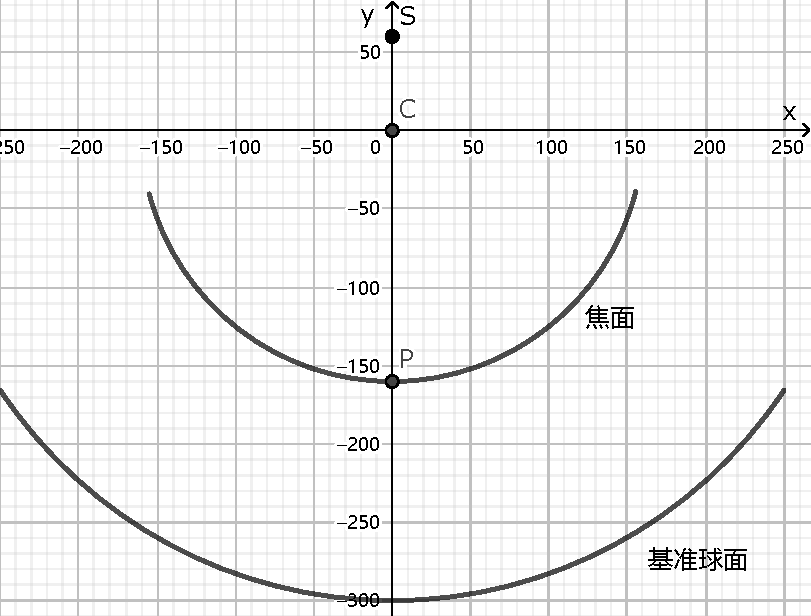
\includegraphics[width=.45\textwidth]{CoordinateSystem1.pdf}
    \caption{坐标系示意图}
    \label{fig:coordinate1}
\end{figure}
坐标系中基准球面的方程为 $x^2 + y^2 = R^2$。反射面板向下伸缩至极限时的方程为
$x^2 + y^2 = (R + 0.6)^2$,向上伸缩至极限时的方程为 $x^2 + y^2 = (R - 0.6)^2$。

设理想抛物面在此平面上投影的方程为 $x^2 = 4p(y + a)$,将其与反射板向上伸缩至极限时的方程联立
\begin{equation}
    \label{eq:firstOriginal}
    \begin{dcases}
        x^2 = 4p(y + a) \\
        x^2 + y^2 = (R - 0.6)^2
    \end{dcases}
\end{equation}
由几何关系可得 $p = a - R * (1 - 0.466)$ 。解方程组 \ref{eq:firstOriginal} 得
\[
    \text{\Large $x =$}
    \begin{dcases}
        -\sqrt{\frac{4\,{\left(5\,a-801\right)}\,{\left(2\,\sqrt{\frac{41295363226730493}
        {34359738368}-4005\,a}-5\,a+1602\right)}}{25}}                    \\
        -\sqrt{-\frac{4\,{\left(5\,a-801\right)}\,{\left(5\,a+2\,\sqrt{
        \frac{41295363226730493}{34359738368}-4005\,a}-1602\right)}}{25}} \\
        \sqrt{\frac{4\,{\left(5\,a-801\right)}\,{\left(2\,\sqrt{\frac{41295363226730493}
        {34359738368}-4005\,a}-5\,a+1602\right)}}{25}}                    \\
        \sqrt{-\frac{4\,{\left(5\,a-801\right)}\,{\left(5\,a+2\,\sqrt{
                            \frac{41295363226730493}{34359738368}-4005\,a}-1602\right)}}{25}}
    \end{dcases}
\]
其中 $a$ 的范围为 $\left[R - 0.6, R + 0.6\right]$。
\subsubsection{模型的解}
在附件中,我们找到一个主节点的坐标为 $(0,0,-300.4)$,结合题目中给出球面半径约为 $300$,
所以 $R = 300.4$。在 $a$ 的取值范围内对 $a$ 进行枚举,得出最优值 $a = 299.90245$。
可算出 $p = 139.4888$,所以得到的理想抛物面的方程为
\[
    x^2 + y^2 = 557.9552(y + 299.90245)
\]
\subsection{问题二}
\subsubsection{模型的建立}

\nocite{宋叶志2019}
\bibliography{references}
\begin{appendices}
    \section{第一问MATLAB代码一}
    \begin{lstlisting}[language=matlab]
syms x p a
equ2 = x^2+(x^2/(4*(a-300.4*0.534))-a)^2-(300.4-0.6)^2==0
[x] = solve(equ2,x)
\end{lstlisting}
    \section{第一问MATLAB代码二}
    \begin{lstlisting}[language=matlab]
f1 = @(a) -sqrt(((35184372088832*a - 5644051790509061)*(sqrt(59671845676091418542400129992729 - 198582418285909280249192906752*a) - 17592186044416*a + 5644051790509061))/154742504910672534362390528);
f3 = @(a) sqrt(((35184372088832*a - 5644051790509061)*(sqrt(59671845676091418542400129992729 - 198582418285909280249192906752*a) - 17592186044416*a + 5644051790509061))/154742504910672534362390528);

ansa = 0;
for a = 300.4-0.6 : 0.00001 : 300.4+0.6
   x = f3(a)-f1(a);
   if(x>300 && abs(ansa-300.4) > abs(a-300.4))
       ansx = x/2
       ansa = a
   end
   x1 = x;
end
R = 300.4;
%ansa = 299.49615
p = ansa - R * 0.534
ansa
\end{lstlisting}
\end{appendices}
\end{document}